\documentclass[11pt]{article}
\usepackage{acl2014}
\usepackage{times}
\usepackage{url}
\usepackage{latexsym}
\usepackage{graphicx}

%\documentclass[10pt]{article}
%\usepackage[margin=1in]{geometry}
\usepackage{amsmath}
\usepackage{amsfonts}
\usepackage{amssymb}
%\usepackage{graphicx}
%\usepackage{natbib}

\title{Inside Outside Recursive Neural Network: A Unified Framework for 
Compositional Semantics and Meaning in Context}
\author{Phong Le, Willem Zuidema}

\begin{document}

\maketitle

%%%%%%%%%%%%%%%%%%%%%%%%%%%%%%%%%%%%%%%%%%

\section{Introduction}
\label{section introduction}

[...]

Firstly, we ask ourselves ``Which evidence is strong enough to be used for 
learning compositional semantics?'' To answer this question, we rely on the 
following observation: a human being can guess the meaning of an unknown 
word by making use of the meaning of its context. In other words, he computes 
(in his brain) the meaning of the context and then use it to predict the meaning 
of the target unknown word (by setting some contrains to narrow down a list of 
possible meanings). Hence, if he correctly predicts the meaning of the unknown word, 
we can, at some level of belief, say that he coherends the meaning of the context. 
This idea is then encaptured in the following hypothesis
\begin{quote}
\textit{Hypothesis 1:} The agreement betwen words and contexts provides evidence for unsupervised 
compositional semantics learning. 
\end{quote}

Then, there are three questions need to be answered in other to implement the 
hypothesis
\begin{enumerate}
	\item How to construct phrasal semantics?
	\item How to construct contextual semantics?
	\item How to use contextual semantics and lexical semantics to learn 
	compositionality functions?
\end{enumerate}
In the next section, we answer these questions.

%%%%%%%%%%%%%%%%%%%%%%%%%%%%%%%%%%%%%%%%%%

\section{Recursive Neural Network (RNN)}
\label{section rnn}
\cite{socher_learning_2010} answer the first question ``How to construct phrasal semantics?'' 
by Recusive Neural Network (RNN) architecture, 
which is used to compute continuous phrase representations. In other to see how RNN works, 
let's conside the following example. Assuming that there is a consitutent with parse
tree $(p_2 \; (p_1 \; x \; y) \; z)$ as in Figure~\ref{figure rnn}. We will use a neural network, 
which contains a weight matrix $\mathbf{W}_1$ for left children and a weight matrix $\mathbf{W}_2$ 
for right children, to compute parents in a bottom up manner. Firstly, we use this network 
to compute $p_1$ based on its children $x$ and $y$
\begin{equation}
	\mathbf{p}_1 = f(\mathbf{W}_1 \mathbf{x} + \mathbf{W}_2 \mathbf{y} + \mathbf{b})
\end{equation}
where $\mathbf{b}$ is a bias, $f$ is an activation function (e.g. \textit{tanh} or \textit{logistic}).
Then, we use the same network to compute $p_2$ based on its children $p_1$ and $z$
\begin{equation}
	\mathbf{p}_2 = f(\mathbf{W}_1 \mathbf{p}_1 + \mathbf{W}_2 \mathbf{z} + \mathbf{b})
\end{equation}
This process is continued until we reach the root node.  This network is trained by 
a gradient-based optimization method (e.g., gradient descent) where the gradient 
over parameters is efficiently computed thanks to the backpropagation through structure
\cite{goller_learning_1996}. Using this architecture 
(and its extensions), Socher and colleagues succesfully reach 
state-of-the-art results in syntactic parsing \cite{socher2013parsing} and 
sentiment analysis \cite{socher2013recursive}. 
\begin{figure}
	\center
	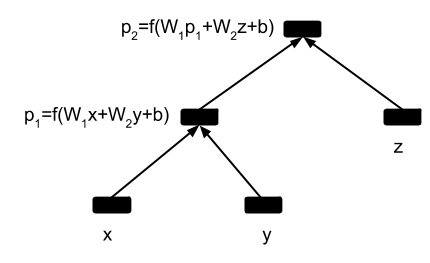
\includegraphics[scale=0.5]{RNN.png}
	\caption{Example of RNN.}
	\label{figure rnn}
\end{figure}

In order to use this architecture in an unsupervised learning manner, 
\cite{socher2011semi} replace neural network in RNN by autoencoder 
(and hence the new architecture is called Recursive Autoencoder - RAE), 
which is a feedforward neural network trained by forcing output equal to 
input (see Figure~\ref{figure rae}). Training a RAE is therefore to minmize 
the sum of reconstruction errors 
(i.e., $\|[\mathbf{x}';\mathbf{y}'] - [\mathbf{x};\mathbf{y}]\|^2$) at all internall nodes. 

\begin{figure}
	\center
	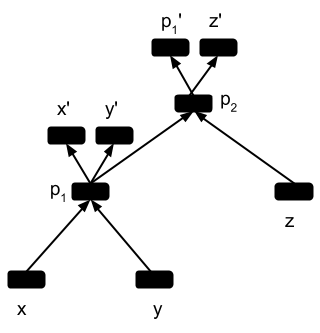
\includegraphics[scale=0.5]{RAE.png}
	\caption{Example of RAE.}
	\label{figure rae}
\end{figure}

%%%%%%%%%%%%%%%%%%%%%%%%%%%%%%%%%%%%%%%%%%

\section{Inside Outside Recursive Neural Network (IORNN)}
\label{section nlm}

None of the above architectures, RAE or RNN, compute contextual semantics. 
However, they give us a hint to do that. In this section, we will answer the second 
question ``How to construct contextual semantics?'' by a new neural network 
architecture, namely Inside Outside Recursive Neural Network (IORNN). We also 
present this architecture by using an example of a constituent and parse tree 
$(p_2 \; (p_1 \; x \; y) \; z)$ (see Figure~\ref{figure iornn}).

\begin{figure}[h!]
	\center
	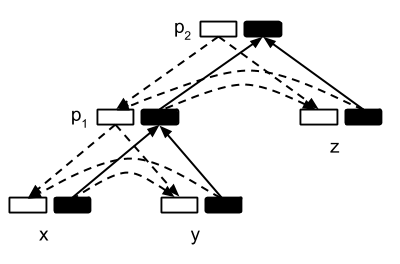
\includegraphics[scale=0.5]{IORNN.png}
	\caption{Inside-Outside Recursive Neural Network. Black rectangles correspond to inner meanings, 
	white rectangles correspond to outer meanings.}
	\label{figure iornn}
\end{figure}


Each node $u$ is assigned two vectors $\mathbf{o}_u$ and $\mathbf{i}_u$. The first one,
called \textit{outer meaning}, denotes the meaning of the context; the second one, 
called \textit{inner meaning}, denotes the meaning of the phrase that the node covers.

\paragraph{Word embeddings} (e.g., $\mathbf{i}_x$)
Similar to \cite{socher_learning_2010}, and \cite{collobert_natural_2011}, given a string of binary
representations of words $(a, b, ..., w)$ (i.e., all of the entries of $w$ are zero except the one 
corresponding to the index of the word in the dictionary), 
we first compute a string of vectors $(\mathbf{i}_{a},...,\mathbf{i}_{w})$ 
representing inner meanings of those words by using 
a look-up table (i.e., word embeddings) $\mathbf{L} \in \mathbb{R}^{n \times |V|}$, 
where $|V|$ is the size of the vocabulary and $n$ is the dimensionality of the vectors. 
This look-up table $\mathbf{L}$ could be seen as a storage of lexical semantics where each column 
is a vector representation of a word. Hence, 
\begin{equation}
    \label{equation compute word vector}
    \mathbf{i}_{w} = \mathbf{L} w \in \mathbb{R}^n
\end{equation}

\paragraph{Computing inner meaning} The inner meaning of a non-terminal node, say $p_1$, is given by
\begin{equation}
	\mathbf{i}_{p_1} = f(\mathbf{W}_1^i \mathbf{i}_{x} + \mathbf{W}_2^i \mathbf{i}_{y} + \mathbf{b}^i)
	\label{equation inner}
\end{equation}
where $\mathbf{W}_1^i, \mathbf{W}_2^i$ are $n \times n$ real matrices, 
$\mathbf{b}^i$ is a bias vector, and $f(.)$ is an activation function, e.g. $tanh$ 
function. Intuitively, the inner meaning of a parent node is the function of the inner meanings 
of its children. This is similar to what \cite{socher_learning_2010} call recursive neural network.

\paragraph{Computing outer meaning} The outer meaning of the root node, $\mathbf{o}_{root}$, is initially 
set randomly, and then learnt later. To a node which is not the root, say $p_1$, the outer meaning is given by
\begin{equation}
	\mathbf{o}_{p_1} = g(\mathbf{W}_1^o \mathbf{o}_{p_2} + \mathbf{W}_2^o \mathbf{i}_{z} + \mathbf{b}^o)
	\label{equation outer}
\end{equation}
where $\mathbf{W}_1^o, \mathbf{W}_2^o$ are $n \times n$ real matrices, 
$\mathbf{b}^o$ is a bias vector, and $g(.)$ is an activation function, e.g. $tanh$ 
function. Informally speaking, the outer meaning of a node (i.e., the meaning of 
its context) is the function of the outer meaning of its parent and the inner meaning 
of its sister. 

The reader, if familiar with syntactic parsing, could recognizes the similarity between 
Equation~\ref{equation inner}, ~\ref{equation outer}
and the inside, outside probabilities given a parse tree.
Therefore, we name the architecture Inside-Outside Recursive Neural Network.

%%%%%%%%%%%%%%%%%%%%%%%%%%%%%%%%%%%%%%%%%%

\section{Training IORNN}
\label{section train iornn}

This section is to answer the final question ``How to use contextual semantics and 
lexical semantics to learn compositionality functions?''. 

According to Hypothesis 1, there must be a strong correlation 
between $\mathbf{o}_{w}$ and $\mathbf{i}_{w}$ where $w$ is any word in 
a given sentence. The simplest way to train the network is to force 
$\mathbf{o}_{w_j} = \mathbf{i}_{w_j}$; hence, learning is to minimize the following 
loss function
\begin{equation}
	J(\theta) = \sum_{s \in D} \sum_{w \in s} \| \mathbf{o}_{w} - \mathbf{i}_{w} \|
\end{equation}
where $D$ is a set of training sentences and $\theta$ are the network parameters. 
However, that could be problematic because 
the meaning of context is not necessary the meaning of the target word.

Here, based on the observation that the meaning of context sets contraints on 
selecting a word to fill in the blank, one could suggest put a \textit{softmax} neuron 
unit on the top of each $\mathbf{o}_w$ in order to compute the probability $P(x|\mathbf{o}_w)$. 
Unfortunately, as pointed out by \cite{collobert_natural_2011}, it might not work. 

Using the same method proposed by \cite{collobert_natural_2011}, we train the network 
such that it gives a higher score to the correct target word rather than to incorrect ones. 
The score $s(x,\mathbf{o}_w)$ given to a candidate word $x$ for a specific context 
$\mathbf{o}_w$ is computed by 
\begin{align}
	u(x,\mathbf{o}_w) & = f(\mathbf{W}_u^o \mathbf{o}_w + \mathbf{W}_u^i \mathbf{i}_x + \mathbf{b}_u) \\
	s(x,\mathbf{o}_w) & = \mathbf{W}_s u(x,\mathbf{o}_w) + \mathbf{b}_s
\end{align}
where $\mathbf{W}_u^o,\mathbf{W}_u^i$ are $n \times k$ real matrices, $ \mathbf{W}_s$ is 
a $k \times 1$ matrix, and $\mathbf{b}_u, \mathbf{b}_s$ are bias vectors. (We fix $k=2n$.) 
Now, the objective function is the ranking criterion with respect to $\theta$
\begin{equation}
	J(\theta) = \sum_{s \in D} \sum_{w \in s} \sum_{x \in V} \max \{0, 1 - s(w,\mathbf{o}_w) + s(x,\mathbf{o}_w) \}
\end{equation}

To minimize the above objective function, we randomly pick up a word 
in the dictionary as a corrupt example, compute the gradient, and update 
the parameters by a gradient descent method. Thanks to the backpropagation 
through structure \cite{goller_learning_1996}, the gradient is efficiently computed. 
Following \cite{socher2013recursive}, we use AdaGrad \cite{duchi2011adaptive}
to update the parameters.

\bibliographystyle{apalike}
\bibliography{ref}

\end{document}
